% $Id: template.tex 11 2007-04-03 22:25:53Z jpeltier $

\documentclass{vgtc}                          % final (conference style)
%\documentclass[review]{vgtc}                 % review
%\documentclass[widereview]{vgtc}             % wide-spaced review
%\documentclass[preprint]{vgtc}               % preprint
%\documentclass[electronic]{vgtc}             % electronic version

%% Uncomment one of the lines above depending on where your paper is
%% in the conference process. ``review'' and ``widereview'' are for review
%% submission, ``preprint'' is for pre-publication, and the final version
%% doesn't use a specific qualifier. Further, ``electronic'' includes
%% hyperreferences for more convenient online viewing.

%% Please use one of the ``review'' options in combination with the
%% assigned online id (see below) ONLY if your paper uses a double blind
%% review process. Some conferences, like IEEE Vis and InfoVis, have NOT
%% in the past.

%% Figures should be in CMYK or Grey scale format, otherwise, colour 
%% shifting may occur during the printing process.

%% These few lines make a distinction between latex and pdflatex calls and they
%% bring in essential packages for graphics and font handling.
%% Note that due to the \DeclareGraphicsExtensions{} call it is no longer necessary
%% to provide the the path and extension of a graphics file:
%% \includegraphics{diamondrule} is completely sufficient.
%%
\ifpdf%                                % if we use pdflatex
  \pdfoutput=1\relax                   % create PDFs from pdfLaTeX
  \pdfcompresslevel=9                  % PDF Compression
  \pdfoptionpdfminorversion=7          % create PDF 1.7
  \ExecuteOptions{pdftex}
  \usepackage{graphicx}                % allow us to embed graphics files
  \DeclareGraphicsExtensions{.pdf,.png,.jpg,.jpeg} % for pdflatex we expect .pdf, .png, or .jpg files
\else%                                 % else we use pure latex
  \ExecuteOptions{dvips}
  \usepackage{graphicx}                % allow us to embed graphics files
  \DeclareGraphicsExtensions{.eps}     % for pure latex we expect eps files
\fi%

%% it is recomended to use ``\autoref{sec:bla}'' instead of ``Fig.~\ref{sec:bla}''
\graphicspath{{figures/}{pictures/}{images/}{./}} % where to search for the images

\usepackage{microtype}                 % use micro-typography (slightly more compact, better to read)
\PassOptionsToPackage{warn}{textcomp}  % to address font issues with \textrightarrow
\usepackage{textcomp}                  % use better special symbols
\usepackage{mathptmx}                  % use matching math font
\usepackage{times}                     % we use Times as the main font
\renewcommand*\ttdefault{txtt}         % a nicer typewriter font
\usepackage{cite}                      % needed to automatically sort the references
\usepackage{tabu}                      % only used for the table example
\usepackage{booktabs}                  % only used for the table example
%% We encourage the use of mathptmx for consistent usage of times font
%% throughout the proceedings. However, if you encounter conflicts
%% with other math-related packages, you may want to disable it.


%% If you are submitting a paper to a conference for review with a double
%% blind reviewing process, please replace the value ``0'' below with your
%% OnlineID. Otherwise, you may safely leave it at ``0''.
\onlineid{0}

%% declare the category of your paper, only shown in review mode
\vgtccategory{Research}

%% allow for this line if you want the electronic option to work properly
\vgtcinsertpkg

%% In preprint mode you may define your own headline.
%\preprinttext{To appear in an IEEE VGTC sponsored conference.}

%% Paper title.

\title{Yelp Rating Prediction Visualization}

%% This is how authors are specified in the conference style

%% Author and Affiliation (single author).
%%\author{Roy G. Biv\thanks{e-mail: roy.g.biv@aol.com}}
%%\affiliation{\scriptsize Allied Widgets Research}

%% Author and Affiliation (multiple authors with single affiliations).
%%\author{Roy G. Biv\thanks{e-mail: roy.g.biv@aol.com} %
%%\and Ed Grimley\thanks{e-mail:ed.grimley@aol.com} %
%%\and Martha Stewart\thanks{e-mail:martha.stewart@marthastewart.com}}
%%\affiliation{\scriptsize Martha Stewart Enterprises \\ Microsoft Research}

%% Author and Affiliation (multiple authors with multiple affiliations)
\author{Jiawen Liu\thanks{e-mail: Jiawen Liu}\\ %
  \and Keke Wu\thanks{e-mail: Keke.Wu@colorado.edu}\\ %
  \and Wei Miao\thanks{e-mail: Wei.Miao@colorado.edu}\\ %
  \and Xu Han\thanks{e-mail: xuha2442@colorado.edu}\\ %
  \and Yawen Zhang\thanks{e-mail: Yawen.Zhang@colorado.edu}\\ %
  }

%% A teaser figure can be included as follows, but is not recommended since
%% the space is now taken up by a full width abstract.
%\teaser{
%  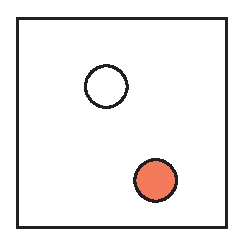
\includegraphics[width=1.5in]{sample.eps}
%  \caption{Lookit! Lookit!}
%}

%% Abstract section.
\abstract{Yelp is a crowd-sourced local business review and social networking community, which has hundreds of thousands of users contribute their data every day. Based on users' reviews and ratings, good local businesses stand out among their categories on top of the list, acting as a word-of-mouth reference. However, tons of user data doesn't make any sense unless we make good use of it. In this case, we decided to look into the problem that how we might get as much as useful information from our data with a particular interest in how the users' rating behavior are influenced by different factors, and what kind of prediction we can make out of the rating pattern we found. With various features extracted from Yelp data, we conducted feature selection, best split and finally built a Decision Tree model which predicts users' rating based on those features. Our visualization includes the complete process of this typical machine learning method, which provides insights about the inner mechanism of how the rating prediction is conducted. %
} % end of abstract

%% ACM Computing Classification System (CCS). 
%% See <http://www.acm.org/about/class> for details.
%% We recommend the 2012 system <http://www.acm.org/about/class/class/2012>
%% For the 2012 system use the ``\CCScatTwelve'' which command takes four arguments.
%% The 1998 system <http://www.acm.org/about/class/class/2012> is still possible
%% For the 1998 system use the ``\CCScat'' which command takes four arguments.
%% In both cases the last two arguments (1998) or last three (2012) can be empty.

\CCScatlist{
  \CCScatTwelve{Yelp}{Rating Prediction}{Decision Tree}{Visualization};
  %\CCScatTwelve{Human-centered computing}{Visu\-al\-iza\-tion}{Visualization design and evaluation methods}{}
}

%\CCScatlist{
  %\CCScat{H.5.2}{User Interfaces}{User Interfaces}{Graphical user interfaces (GUI)}{};
  %\CCScat{H.5.m}{Information Interfaces and Presentation}{Miscellaneous}{}{}
%}

%% Copyright space is enabled by default as required by guidelines.
%% It is disabled by the 'review' option or via the following command:
% \nocopyrightspace

%%%%%%%%%%%%%%%%%%%%%%%%%%%%%%%%%%%%%%%%%%%%%%%%%%%%%%%%%%%%%%%%
%%%%%%%%%%%%%%%%%%%%%% START OF THE PAPER %%%%%%%%%%%%%%%%%%%%%%
%%%%%%%%%%%%%%%%%%%%%%%%%%%%%%%%%%%%%%%%%%%%%%%%%%%%%%%%%%%%%%%%%

\begin{document}

%% The ``\maketitle'' command must be the first command after the
%% ``\begin{document}'' command. It prepares and prints the title block.

%% the only exception to this rule is the \firstsection command
\firstsection{Introduction}

\maketitle

%% \section{Introduction} %for journal use above \firstsection{..} instead
Rating prediction plays an important role in the recommendation system as to capture users' preference for specific product. In Yelp, user can post their rating and review for a restaurant they visited, and these data as well as user/restaurant related attributes, e.g., user average rating, restaurant location or category, can be well gathered for conducting the rating prediction. If a user's rating for a restaurant can be accurately predicted, Yelp would be able to recommend high rating product to the user which meets their preferences. 

The challenge in this problem lies in the feature selection and modeling processing. With multiple features related to a user's rating, picking up the effective features is quite important, which would significantly influence the prediction performance. Additionally, the modeling process which selects the best machine learning model for rating prediction is also critical, and it's necessary to gain insights about how the model functions, i.e., the inner mechanism of model. Previously, most machine learning processes have been conducted in a "black box", by just showing input and output. In our project, we aim at visualizing the whole process, including feature selection, best split, and model tree. The Decision Tree model is selected because its straightforward idea in classification, which would be beneficial for visualization. 

\section{Related Work}

In this project, we deploy the visualization principles and techniques to make mechanism of the whole recommendation system(RS) transparent based on Yelp's public dataset\cite{yelpdata}. A lot of research has been done on recommendation system and the RS techniques are broadly divided into two types: memory-based approach, which recommend business based on similarity or correlation between users\cite{sarwar2001item}, and model-based approach, which use machine learning methods to predict user ratings\cite{portugal2017use}. In our project, we use decision tree from model-based approach\cite{cho2002personalized} as our visualization example. 

Our visualization of modeling process mainly focus on four parts: feature engineering, best split analysis, feature ranking and model training. For feature engineering, we extract 22 features in total, includes user-related features(7), business-related features(3), user-category features(5) and review-related features(7). Among review-related features, we extract several advanced natural language processing(NLP) features like polarity\cite{das2012sentimantics} and subjectivity\cite{montoyo2012subjectivity}. For best spllit analysis, we create a moveable threshold to study how this feature -- business average star, could influence the decision making(whether to recommend or not). When moving the threshold, the calculated accuracy and true positive rate\cite{spackman1989signal} will be changed correspondingly and we can choose the threshold with highest accuracy as our decision tree's best split. In the part of feature ranking, we measure the importance of all 22 features based on the score retrieved by Xgboost\cite{chen2016xgboost}. Xgboost's feature importance method calculateds F score, which indicates how many times the feature split on. Higher the F score is, more important the feature is. In our feature ranking visualization, we use a radar graph to show the importance of all these features based on F score. The last step is model training, we use 100 users as an example. 80 users are used to train and 20 users are used to test. The top three features with highest F score are selected and used by the model. We visualize each users path and the overall test accuracy.

\section{Design Process}

During the design process, we tried to get our results displayed in a reader-driven rather than author-driven way, following a storytelling style. Our preliminary works included data cleaning, data organization by categories, feature selection, hand-written sketches of the complete workflow. We used web as our platform and D3.js as the main tool. The web was divided into six different but consistent sections in the order of Our Story, Our Goal, Our Design, Visualization, Split and Tree Model, which was exactly the sequence we were following to dive into this topic. In terms of the visual design, we used the red, black and white color scheme adopted by Yelp to make it look consistent. Besides text descriptions and interactive visualization graphs, we also had hand-written sketches on the web as a proof of concept, which helped enrich the design elements' diversity. In terms of the visualization design, we used four different types of charts to visualize four different rating related data features. The restaurant ratings by category were visualized in a bar chart, showing customers' preferences on cuisines. The average ratings by state were visualized in a US map, with the darker colored state having a higher rating trend. We also extracted key words from users' reviews and got them displayed in a randomly generated word cloud, where the words were extinguished from each other by five colors mapped with five different rating stars. Besides these, we also built a network to visualize the influence on ratings from Yelp users who have most friends. All of these charts were interactive and dynamic, enabling a good user-directed exploration experience. Following sections utilized a split framework to explain how we applied machine learning to help us make predictions. Finally, a decision-tree like model walked the audience through the decision and prediction making process. With a well-designed and fully-interactive design style, we hope to help our audience get valuable information in a way that can be adjusted as they like. Meanwhile, we hope to use some vivid graphs and animations to bridge the gap between scientific research and general public understanding, making the abstract concept intuitive and straightforward.


\section{Modeling Process}


For Yelp rating prediction, we use Decision Tree, which is tree-like graph of decisions and their possible consequences. It is widely used prediction model in machine learning. In this tree structure, leaves represent class labels and branches represent conjunctions of features that lead to the class labels. The modeling process include feature selection, best split, feature ranking and tree generation. 

\paragraph{Feature Selection}
%There are multiple features related a user's rating. \textcolor{red}{give list or table, showing all features. }
Yelp dataset contains 11 tables such as Yelp dataset contains 11 tables such as business, category, checkin, etc. Figure \ref{fig:data}\footnote{\url{https://www.yelp.com/dataset/documentation/sql}} shows the dataset structure. We extract 22 features(shown in Table \ref{tb:feature}, which could be divided into four groups: user-related features(7), business-related features(3), user-category features(5) and review-related features(7).

%-------------------------------------------
\begin{figure}[h]
  \centering
  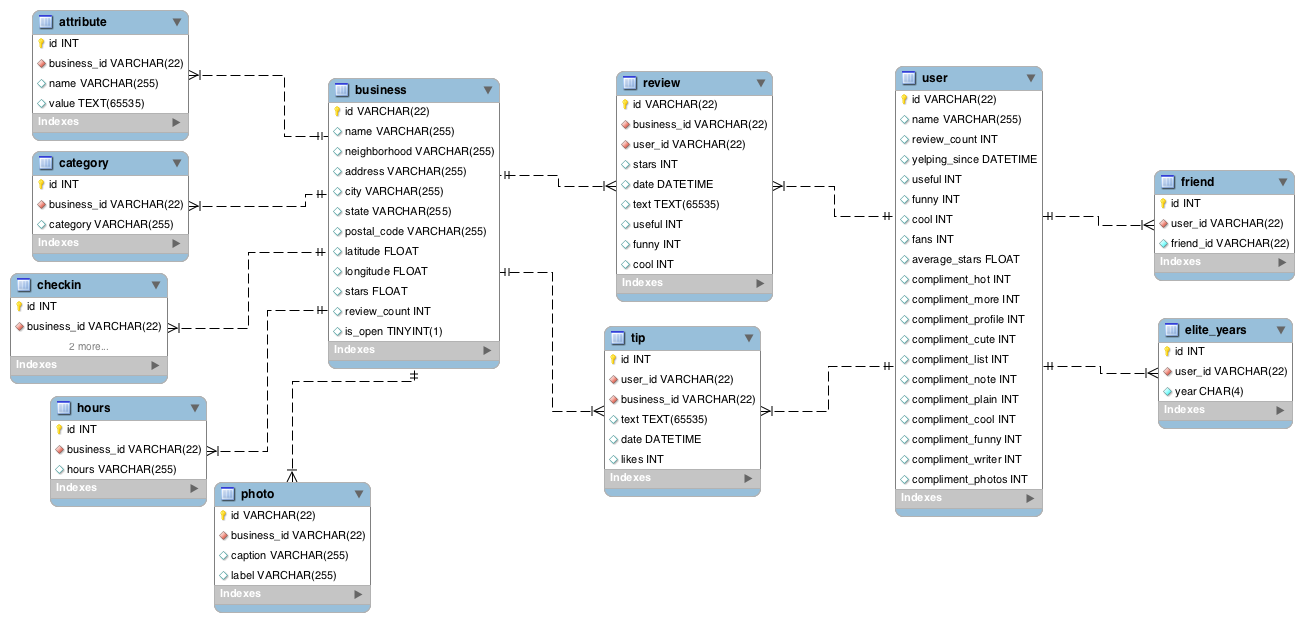
\includegraphics[width=6cm]{data.png}
  \caption{The structure of Yelp Dataset}
  \label{fig:data}
\end{figure}
%------------------------------------------- 
\newcommand{\tabincell}[2]{\begin{tabular}{@{}#1@{}}#2\end{tabular}}
\begin{table}
\centering
\caption{Feature Groups}
\label{tb:feature}
\begin{tabular}{|c|c|}
\hline
Feature Group & Features \\ \hline
\tabincell{c}{User-related \\Features(7)} & \tabincell{c}{user compliment count\\user funny count\\user cool count\\user useful count\\user fans count \\ user review count \\ user average rating} \\ \hline
\tabincell{c}{Business-related \\Features(3)} & \tabincell{c}{business average rating\\business location-related rating\\business neighborhood-related rating} \\ \hline
\tabincell{c}{Review-related \\Features(7)} & \tabincell{c}{Polarity \\  Subjectivity  \\  TF-IDF  \\ Meaningful word count  \\ review useful count\\ review cool count \\ review funny count  } \\  \hline
\tabincell{c}{User-category \\Features(5)} & \tabincell{c}{  uc-review count   \\  uc-average rating  \\ uc-review funny count \\  uc-review  cool count   \\  uc-review useful count }\\
\hline
\end{tabular}
\end{table}


\paragraph{Best Split}
Decision Tree works in a top-down manner, we need to choose a variable at each step that best split the sets of items. The best split are chosen by certain metric, e.g., Gini impurity, Information gain and so on. 

\paragraph{Feature Ranking}
Feature ranking helps us have a better understanding of how each feature contribute to our model training. Table \ref{tb:ranking} shows the result of our 22 feature ranking. From this table we can know that review's polarity, user to a certain category's average rating, user to a certain category's review count.

\begin{table}[h]
  \small
  \centering
  \caption{Feature Ranking Results}
  \label{tb:ranking}
  \begin{tabular}{l|l}
    \hline
    \textbf{Feature}                          & \textbf{F score (scaled)}                                                                \\ \hline
    polarity     & 85                       \\ \hline
    uc-average rating      & 67                        \\ \hline
    uc-review count & 42\\ \hline
    subjectivity & 42\\ \hline
    business average rating & 29\\ \hline
    user average rating & 26\\ \hline
    user useful count & 16\\ \hline
    review useful count     & 16                       \\ \hline
    TF-IDF      & 16                        \\ \hline
    user review count & 16\\ \hline
    user compliment count & 14\\ \hline
    review cool count & 11\\ \hline
    review funny count & 10\\ \hline
    uc-review useful count& 8\\ \hline
    user funny count & 8\\ \hline
    user fans count     & 6                       \\ \hline
    user cool count      & 4                        \\ \hline
    uc-review cool count & 2\\ \hline
    uc-review funny count & 1\\ \hline
    business location-related rating & 1\\ \hline
    business neighborhood-related rating & 1\\ \hline
    meaningful word count& 1\\ \hline

  \end{tabular}
\end{table}


\paragraph{Tree Generation}
With the selected features, and variables chosen by best split, a tree can be generated. And each path in the tree represents a decision-making process, in which a user's rating can be predicted based on a series of decision makings. Here we use only 80 users to train our model. Under this situation, even though the generated decision tree has really simple structure and only top three features are involved, the trained model could still have high prediction accuracy(100\%).

\section{Results}

Our visualization storyline include four parts, features, best split, feature ranking and tree model. 

\subsection{Vis 1: Features}

In this part, as shown in Figure \ref{fig:vis_1}, we selected four typical features related to users' rating, including 1) restaurant type, visualized with a bar chart, 2) restaurant location, visualized with a map, 3) frequent words related to different ratings, visualized with a word cloud, 4) friendship network, visualized with a network. With these four selected features and different visualizations, we aimed to illustrate the difference of features. In each visualization, we added the rating information by either using the tooltip or other methods to show how the features are related to user's rating. 

%-------------------------------------------
\begin{figure}[h]
  \centering
  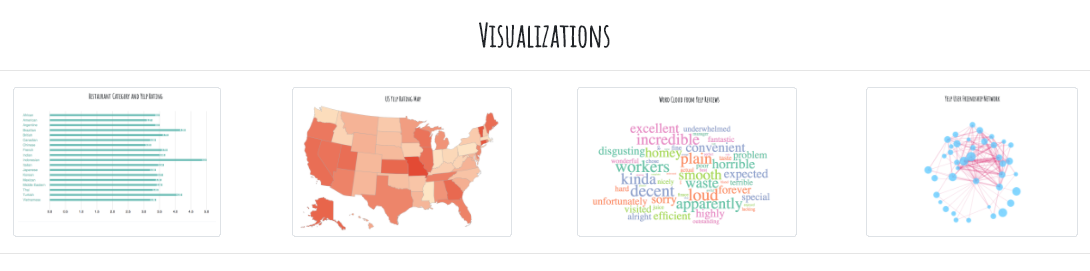
\includegraphics[width=9cm]{vis_1.png}
  \caption{Visualizations of selected features related to users' rating.}
  \label{fig:vis_1}
\end{figure}
%------------------------------------------- 

\subsection{Vis 2: Best Split}

As to demonstrate how different cut-offs would influence the prediction results, we used user's average rating as an example, to illustrate the influence of thresholds on correct and other rates in the prediction results. The best split is determined by choosing the right threshold of the feature. As shown in Figure \ref{fig:vis_2}, when the threshold of user average rating is changed, the correct, incorrect, true positive, positive rate would all change. We build this visualization based on \cite{bestsplit}.For all the features used for rating prediction, their best splits would be determined in advance. 


%-------------------------------------------
\begin{figure}[h]
  \centering
  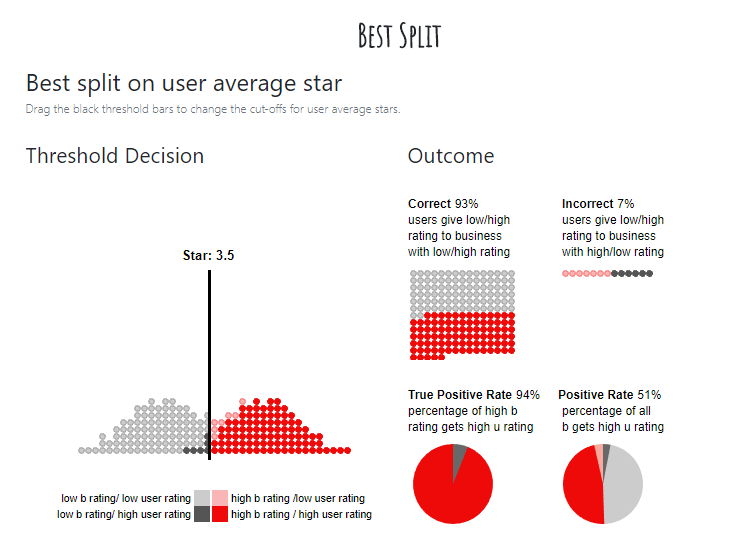
\includegraphics[width=9cm]{vis_2.png}
  \caption{Visualizations of how to choose best split.}
  \label{fig:vis_2}
\end{figure}
%------------------------------------------- 

\subsection{Vis 3: Feature Ranking}

As shown in Figure \ref{fig:vis_3}, with the feature ranking results shown in Table \ref{tb:ranking}, we further visualize the result using an radar map. This map illustrate the importance of different features in rating prediction. This is an important process before generating the tree model as only high ranked features would be used in the tree model. 

%-------------------------------------------
\begin{figure}[h]
  \centering
  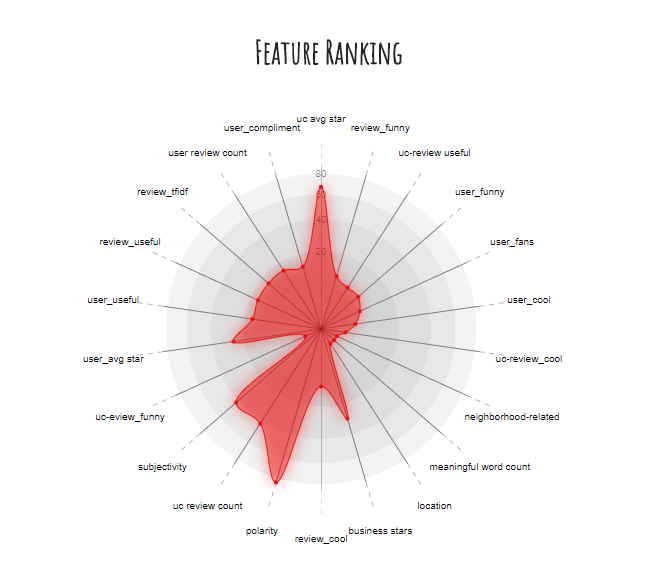
\includegraphics[width=9cm]{vis_3.png}
  \caption{Visualizations of feature ranking result.}
  \label{fig:vis_3}
\end{figure}
%------------------------------------------- 

%-------------------------------------------
\begin{figure}[h]
  \centering
  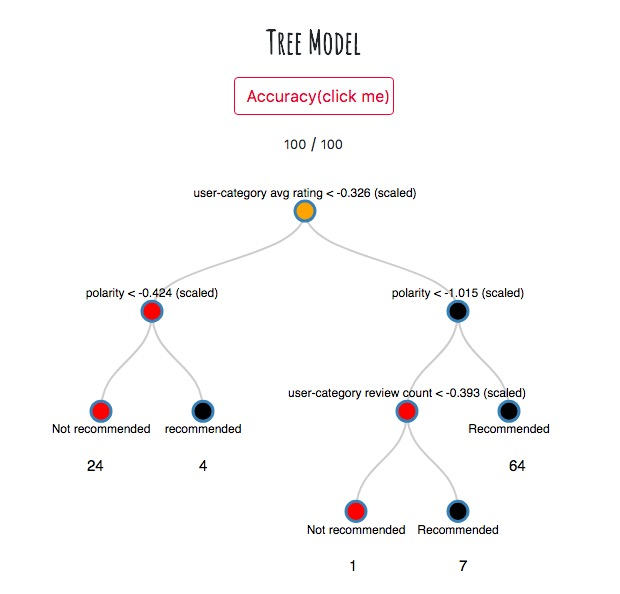
\includegraphics[width=9cm]{vis_4.jpg}
  \caption{Visualizations of tree model and training/test accuracy.}
  \label{fig:vis_4}
\end{figure}
%-------------------------------------------

\subsection{Vis 4: Tree Model}

Finally, with selected features from ranking, we built the decision tree model for rating prediction as shown in Figure \ref{fig:vis_4}. This visualization include the basic tree model with nodes represent the class labels and edges represent conjunctions of feature that lead to the class labels. This tree map works in a dynamic way of showing how a given input would be classified, i.e., how a user's rating would be predicted given related features. Additionally, the training and test accuracy are also calculated. 




\section{Discussion}

In the project, we conducted a visualization of Yelp rating prediction. This visualization not only visualize the data but also visualize the machine learning process, as to reveal information in the "black box". With four parts of visualization, 1) features, 2) best split, 3) feature ranking, 4) tree model, we can understand the Decision Tree model better and gain insights of each part through visualizations. 


%% if specified like this the section will be committed in review mode
\acknowledgments{
We want to thank Prof.Szafir and our teaching assistant Jim Dykes for their inspiring guidance and kind help.}
%\bibliographystyle{abbrv}
\bibliographystyle{abbrv-doi}
%\bibliographystyle{abbrv-doi-narrow}
%\bibliographystyle{abbrv-doi-hyperref}
%\bibliographystyle{abbrv-doi-hyperref-narrow}

\bibliography{template}
\end{document}
